% This is not a step-by-step instruction or diary to your work.
% Instead, you should describe your technical approach and solution, describe architecture, components, etc.
% Think software engineering...
% Perhaps use a few useful uml-diagrams or illustrate the system architecture.
% Keep in mind that the purpose of the implementation section is to describe your implementation to solve the problems from 1.3.
 
% This section can have a lot of subsections, example:
% 4.1 System architecture / System arkitektur
% 4.2 System components / System komponenter
% 4.3 ...

The implementation is separated into three different smaller projects.
The first being a debug library called \emph{rust-debug}.
This library simplifies the process of retrieving debug information from the \gls{DWARF} format.
The second project is the debugger \gls{erdb} and the last one is a \emph{VSCode} extension for \gls{erdb}.


\section{Debugging Library \emph{rust-debug}}
\label{section:rust-debug}
% Explain the implementation of the library rust-debug

% Explain why this library was made.
Retrieving debug information from the \gls{DWARF} sections in the \gls{elf} file is one of the main problems that needs to be solved when creating a debugger.
The \emph{Rust} library \emph{gimli-rs} simplifies that problem by providing data structures and functions for reading the \gls{DWARF} sections.
However, the library requires a lot of knowledge about the \gls{DWARF} format to use.
Thus, the \emph{rust-debug} library was created to make it even easier to get the debug information.
Figure \ref{fig:rustdebug} shows how the two libraries and the \gls{elf} file are connected.


\begin{figure}[h]
	\centering
	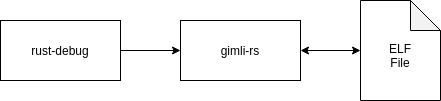
\includegraphics[width=1.0\textwidth]{rust_debug.png}
	\caption{A diagram showing the relation between the \emph{ELF} file and the two libraries \emph{rust-debug} and \emph{gimli-rs}.}
	\label{fig:rustdebug}
\end{figure}


Some of the main functionality that \emph{rust-debug} provides are the following:

\begin{itemize}
  \item Retrieving the source file location for functions, variables, types and more.
  \item Virtually unwinding the call stack.
  \item Evaluating variables.
  \item Translating source file line number to the nearest machine code address.
  \item Finding the \gls{die} that represents a function using the name.
\end{itemize}

There are more functionalities that \emph{rust-debug} provides, but they are not noteworthy.
The code of this library is in the \emph{GIT} repository \cite{rust-debug}.



\subsection{Retrieving Source File Location}
% Explain the evaluation of source information % TODO
Some \glspl{die} in \gls{DWARF} have attributes that starts with \emph{DW\_AT\_decl\_}.
These attributes contain information on where in the source file the \gls{die} was declared.
This includes file path, line number and column number.
The library \emph{rust-debug} has a function for retrieving the value of all these attributes from a given \gls{die}.


The attribute  \emph{DW\_AT\_decl\_file} which contain the file path of where the \gls{die} was declared has a file index as its value.
Every compilation unit has a line number information table that contain file paths which are indexed.
Thus, the \emph{rust-debug} library will search for the matching index in the table to find the file path.
Finding the line and column number does not require any lookup.


\subsection{Accessing Memory And Registers}
% Explain the evaluation part. % TODO
% Explain the stored target memory and registers
One of the requirements for evaluating the value of a variable is access to the registers and memory of the debug target.
\emph{rust-debug} does not have that functionality because it should be hardware independent as much as possible.
Instead, the library uses a data structure which contain the values of the registers and memory.
This keeps the library hardware independent.
The data structure also has some function for reading and adding values.
Thus, it is the user of the library that has to add the values to the data structure.


The register and memory data structure is used as an argument to the functions in the library.
If a value is missing, the called function will return a result that describes which value is missing.
Then the user of the library can read that value from the debug target, and add it to the data structure.
If there are more values missing then calling the function with the updated values will signal that additional values needs to be added.
This repeats until the function give a result that says it has completed its task.


\subsection{Evaluating Variables} \label{sec:ievalvar}
% Explain the evaluation of variables.
The \emph{rust-debug} library has a structure called \emph{VariableCreator}, it takes a reference to a \gls{DWARF} unit and \gls{die}.
The \gls{die} has to be one that represents a variable.
When the data structure is created, it will extract some important information about the variable from the \gls{die}. A constructed \emph{VariableCreator} struct has a method for evaluating the value of the variable that requires the register and memory data structure.
This method evaluates the variable as described in section \ref{sec:evaluate-variable} and the \gls{DWARF} specification \cite{dwarf}.
The return value of the method is an enum that is used for telling the user if a value is missing from the register and memory data structure or not.
Then there exists another method for retrieving the variable information containing the evaluated value.
The variable information contains the following:

\begin{itemize}
  \item Variable name.
  \item Variable type.
  \item Variable location in the source file.
  \item The locations of the variable value in registers and memory.
  \item The evaluated value of the variable.
\end{itemize}


\subsection{Finding a functions DIE} \label{sec:funcdie}
The \emph{rust-debug} library has a function for finding a \gls{die} that represents a function using the name of that function.
The function also needs a machine code address to find the correct compilation unit.


The correct compilation unit can be found using a code address.
Every compilation unit has an address range that can be used to see if the machine code is from that compilation unit.
Thus searching for the correct one is done by going through each unit, and checking if the address is in the range.


When the compilation unit is known, the \gls{die} representing the subroutine can be found by searching the \gls{die} tree of the unit.
This is done by going down the path of the tree where the machine code address is in range.
It returns a result when it has found the subroutine \gls{die} with the searched name, or when there are no more \glspl{die} to check.


\subsection{Unwinding Call Stack}
% Explain the evaluation of call stack % TODO
% Explain the evaluation of stackframe 
The \emph{rust-debug} library has a data structure called \emph{Stacktrace}, which works very similarly to the data structure describe in section \ref{sec:ievalvar}.
However, \emph{Stacktrace} is used to virtually unwind the call stack and evaluate all the variables in it.
The call stack is unwound as described in section \ref{sec:stacktrace} and the \gls{DWARF} specification \cite{dwarf}.
This results in a stack of activations, which most importantly contain restored register values and stack pointers.


All the variables in each of the activations are then evaluated using the restored register values.
This is done using a data structure that works similar to the data structure describe in section \ref{sec:ievalvar}.

The first step of evaluating the variables is finding the \gls{die} of the subroutine that the activation is related to.
This is done using the function described in section \ref{sec:funcdie}.
After that the \gls{die} tree is searched through for variable \glspl{die}, starting at the subroutine \gls{die}.
All the variable \glspl{die} found are added to a list.
Each variable in the list is then evaluated as described in section \ref{sec:ievalvar}.
If there is a missing value from memory then the response from the evaluation of the variable is returned.
Because the data structure works similar to the one in section \ref{sec:ievalvar}, it can continue from where it last stopped.


\subsection{Finding Breakpoint Location}
% Explain how to get breakpoint location.
The \emph{rust-debug} library has a function that finds a machine code location using a source file location.
This machine code location is the closest one that represents the line in the source code.
The function requires a file path and line number, but it also can take a column number.


The mentioned function works by first finding out which compilation unit contains information on the inputted file path.
It does this by looping through all the file entries in the line number information table for every compilation unit.
Each line number information table entry have rows that each contain information on a line from the source code.
Thus, all the rows with the search line numbers are added to a list.
The machine code address of the first element in this list is returned if no column line was inputted to the function.
Otherwise, it is the one with the closest column number that is returned.




\section{Embedded Rust Debugger}
% Explain the genral stucture of the debugger
The debugger \acrfull{erdb} is implemented using the debugging library \emph{rust-debug}.
That library provides all the needed functionalities for retrieving debug information from the \gls{DWARF} format.
The debugger also uses the \emph{probe-rs} library for controlling the \gls{mcu}.
It is also used for accessing the registers and memory of the \gls{mcu}.


The debugger is made up of three modules, the first one is called \acrshort{cli}.
Its main functionality is to handle the input from the console and the output to it.
The second module is called \emph{DebugAdapter}.
It also handles the input and output, but in the form of \gls{dap} messages.
This module is for supporting \glspl{gui} that use the \gls{dap} protocol to display debug information.
The last module is called Debugger, and it runs in a separate thread from the other two modules.
This is the module that uses the \emph{rust-debug} and \emph{probe-rs} library to get debug information.
It is also used to control the debug target.
Figure \ref{fig:ERDStruct} shows a diagram of how these modules are structured.
Also, all the code for \gls{erdb} can be found in this git repository \cite{erdb}.


\begin{figure}[h]
	\centering
	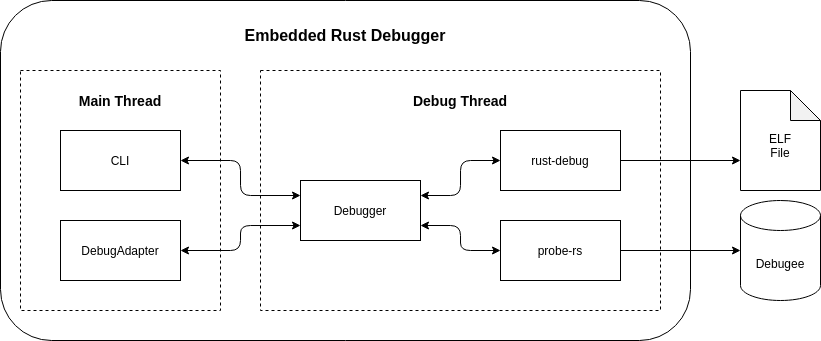
\includegraphics[width=1.0\textwidth]{debugger_structure.png}
	\caption{Diagram showing the structure of ERD.}
	\label{fig:ERDStruct}
\end{figure}


\subsection{The CLI module}
% Explain how the CLI is implemented.
The \emph{CLI} is a very simple one, that has a separate thread for reading the input called the input thread.
The input is read from the console constantly until the user enters a line of text.
Then the inputted line is sent to the main thread.
After that the input thread waits for a response, the type of the response is boolean.
If the response boolean is true then the program will stop, otherwise it starts reading the console for new input again.
The input thread repeats this process until the main thread stops it.


When the main thread receives a message from the input thread it tries to parse it into command.
The parser works by matching the first word in the input with the names of the commands.
If there is a match the commands specific parser is used to parse the rest of the input.
After a command is parsed, it is sent to the debug thread asynchronously.
The main thread then waits for a response from the debug thread, when the response is received the main thread prints it to the console.
After that it sends a response to the input thread and awaits new messages from both the input thread and the debug thread.


An example of all the communication between the user and the threads can be seen in figure \ref{fig:cliflow}.
The example also shows what happens when an event is sent from the debug thread to the main thread.
An event is a message telling the debugger that the debug target has change state from running to stopped or vice versa.


\begin{figure}[h]
	\centering
	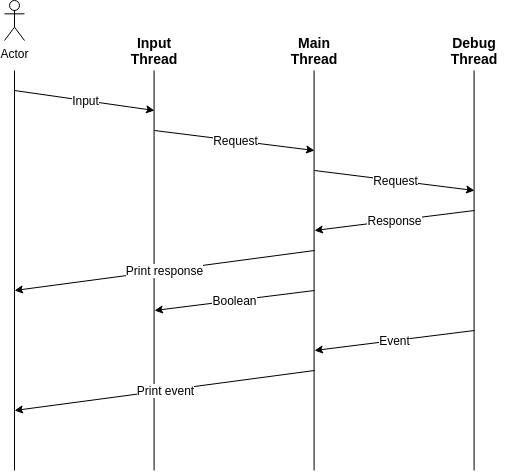
\includegraphics[width=0.9\textwidth]{cli_flow.png}
	\caption{A diagram showing the communication between the user/actor and the three different threads.}
	\label{fig:cliflow}
\end{figure}




\subsection{The Debug Adapter module}
% Explain the implementaiton of the debug adapeter


% Overview description of the debug adapter and the flow of communication from the user to the debugger.
The debug adapter is implemented as a \gls{tcp} server in the main thread.
When a new \gls{tcp} connection is made the debug thread is started.
After it has started the main thread starts listening for \gls{dap} messages on the \gls{tcp} connection.


The first \gls{dap} messages are for communicating the \gls{dap} functionalities that the client and the debugger has.
These first \gls{dap} messages also contain some configuration for debugger module in the debug thread, those configuration are forwarded to the debug thread.
After that the debug adapter will continuously pull for messages from the \gls{tcp} client and the debug thread, until a message is received.


When the debug adapter receives a \gls{dap} message from the client, it is translated into one or more commands.
Those commands are then sent one by one to the debugger module in the debug thread.
The responses from those commands are then used to make a response to the clients \gls{dap} message.
If the debug adapter gets an event from the debug thread, the debug adapter will translate it into a \gls{dap} message and send it to the client.



%% Add a flow cart of the communication? % TODO
%\begin{figure}[h]
%	\centering
%	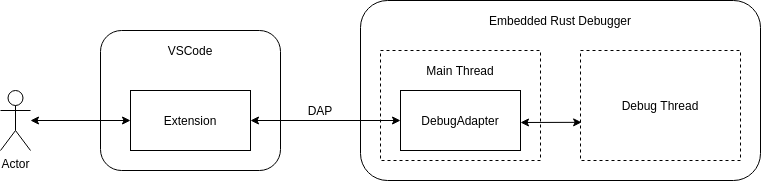
\includegraphics[width=0.9\textwidth]{user_dap_debug.png}
%	\caption{A diagram showing the comunication between the user/actor, \emph{VSCode} and the debugger \emph{Embedded Rust Debugger}.}
%	\label{fig:userDAP}
%\end{figure}





\subsection{The Debugger Module}
The debugger module is designed as a server that listens for commands through a channel.
It is running in a separate thread from the \acrshort{cli} and the debug adapter, which is called the debug thread.
There are two states in which the debug thread can be in, that is in the attached or detached state.
The two states are different in that the attached state can access the debug target and the \gls{DWARF} file.


The debug thread is started by the main thread and starts in the detached state.
In the detached state only the configuration and exit commands work.
The other commands require that the debug target is attached.
But if one of those commands is received then the debug thread will try to enter the attached state.
This can only happen if all the required configuration are set.
If one of the configuration are missing then an error will be sent as a response.


When the debug thread is in the attached state it can use the \emph{rust-debug} library to retrieve debug information.
It can also use the \emph{probe-rs} library for controlling the debug target and reading the registers and memory.
The relation between the libraries can be seen in figure \ref{fig:debugger}.


\begin{figure}[h]
	\centering
	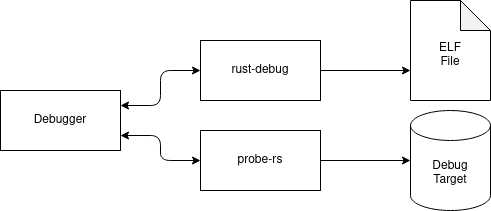
\includegraphics[width=1.0\textwidth]{debugger.png}
	\caption{A diagram showing the relations between the debugger, the \emph{ELF} file, the debug target and the two libraries \emph{rust-debug} and \emph{probe-rs}.}
	\label{fig:debugger}
\end{figure}


\subsubsection{Retrieving Debug Information}
The debugger module retrieves debug information by using the \emph{rust-debug} library.
This library sometimes requires a data structure that contain the values of some registers and memory addresses.
Those function will return an enum that tells if a value is needed and where that value is located.
Thus, the debugger module will use the \emph{probe-rs} library to read the needed value, which is then added to the data structure.
This repeats until no more values are needed, and the result of the evaluation can be retrieved.
The values in the data structure are removed every time the debug target starts executing again.
This is such that no old values are used, and it works because the debug target must be stopped to use related commands.



\subsubsection{Simultaneous Handling of Requests And Events}
% How the debugger handles request and events simultaneously.
The debug thread polls the channel for incoming request and the state of the debug target.
This enables the debug thread to simultaneously handle requests from the user, and events from the debug target.
There is a boolean that keeps track if the debug target is running.
It is used to stop the pulling of the targets state when the debug target is stopped.
This is done because the debug target cannot start executing on its own.


\subsubsection{Optimization of Repeated Variable Evaluation}
% How it handles request for stackframes and variables.
To improve on the performance of the debugger it will temporarily store the values of the stack trace.
This allows for fast repetitive lookup of information present in the stack trace.
The stored stack trace is removed any time the debug target starts executing again.
This ensures that it always gives the correct values and not the old ones.


Note that if a request is received to evaluate one variable, the debugger will then perform a stack trace instead, or read from the temporarily stored stack trace.
This simplifies the implementation a lot and also makes the subsequent evaluation requests faster.


\section{VSCode Extension}
% Explain the implementation of the vscode explanation.
Creating a \emph{VSCode} extension is simple because \emph{Microsoft} has a tool called \emph{TODO} \ref{TODO}, that will generate a empty extension.
They also have a lot of documentation on how to get started with creating a extension.
The documentation mentions how to create debug extensions.
There is two different types of debug extensions, the first is a extension that implements a debug adapter for a specific debugger.
These often require a lot work because a debug adapter needs to translate the \gls{dap} protocol messages to command that the debugger understands.
Thus, depending on the debugger it can require a lot of work to get this working well.
The other type of debug extension is just a wrapper for the debugger that already implements the \gls{dap} protocol.
These extension are very simple to create because the they only need to start the debugger and connect to it using the \emph{dap} protocol.
I refer the reader to \emph{Microsofts} documentations \ref{TODO} for further reading.

The debugger \emph{Embedded Rust Debugger} implements the \gls{dap} protocol over a \gls{tcp} server.
Thus, the \emph{VSCode} extension is just a wrapper that starts the debugger \gls{tcp} server and then connects to it.
Connecting to the debugger server over \gls{tcp} is very easy to do, because \emph{Microsoft} has a library called \emph{VSCode} that does that for you.
The extension also captures the logs of the debugger and outputs them to the user using the \emph{VSCode} library.

There are also some configurations that the user of the \emph{Embedded Rust Debugger} can set in the \emph{launch.json} file.
The available configurations are defined in a \emph{json} file called \emph{TODO} in the extension project.
